\newcommand{\freshResultsAucTable}{
    \begin{center}
        \begin{longtable}[c]{|p{2,8cm}||p{2,8cm} p{2,8cm} p{2,8cm}|}
            \hline
            AUC-ROC & ALOHA & Joint Embedding & Proposed Model \\
            \hline
            \endfirsthead

            \caption*{\raggedright ...continued from previous page} \\
            \hline
            AUC-ROC & ALOHA & Joint Embedding & Proposed Model \\
            \hline
            \endhead

            \caption*{\raggedleft ...continued on next page} \\
            \endfoot

            \caption{Mean and standard deviation AUC-ROC (Area Under Curve) of the different models for the the prediction of the different families on fresh dataset samples. Results were aggregated over \textBF{3} training runs with different weight initializations and minibatch orderings. Best results are shown in \textbf{bold}.} \label{tab:families_aucs}
            \endlastfoot

            Agenttesla & - & 0.506$\pm$0.007 & \textBF{0.516$\pm$0.001} \\
            Avemariarat & - & 0.502$\pm$0.006 & \textBF{0.503$\pm$0.009} \\
            Azorult & - & \textBF{0.500$\pm$0.004} & 0.498$\pm$0.004 \\
            Formbook & - & \textBF{0.503$\pm$0.003} & 0.500$\pm$0.005 \\
            Heodo & - & \textBF{0.519$\pm$0.013} & 0.517$\pm$0.006 \\
            Loki & - & \textBF{0.520$\pm$0.014} & 0.512$\pm$0.002 \\
            Masslogger & - & 0.481$\pm$0.019 & \textBF{0.485$\pm$0.018} \\
            Netwire & - & 0.502$\pm$0.002 & \textBF{0.508$\pm$0.008} \\
            Njrat & - & 0.486$\pm$0.006 & \textBF{0.495$\pm$0.007} \\
            Remcorsat & - & 0.507$\pm$0.004 & \textBF{0.508$\pm$0.004} \\
            \hline
        \end{longtable}
    \end{center}
}

\newcommand{\freshResultsSummaryTable}{
    \begin{center}
        \begin{longtable}[c]{|p{3,2cm}||p{1,8cm} p{1,8cm} p{1,8cm} p{1,8cm} p{1,8cm}|}
            \hline
            & TPR & Accuracy & Precision & Recall & F1 score \\
            \hline
            \endfirsthead

            \caption*{\raggedright ...continued from previous page} \\
            \hline
            & TPR & Accuracy & Precision & Recall & F1 score \\
            \hline
            \endhead

            \caption*{\raggedleft ...continued on next page} \\
            \endfoot

            \caption{Summary of the mean and standard deviation results of the different models for the prediction of the different families on fresh dataset samples at \textbf{FPR} $=1\%$. Results were aggregated over \textBF{3} training runs with different weight initializations and minibatch orderings. Best results are shown in \textbf{bold}.} \label{tab:fresh_results_summary}
            \endlastfoot

            \multicolumn{6}{|c|}{\textbf{Agenttesla} (at FPR $=1\%$)} \\
            \hline
            Joint Embedding & \textBF{0.010$\pm$0.000} & \textBF{0.900$\pm$0.000} & \textBF{1.000$\pm$0.000} & \textBF{0.000$\pm$0.000} & \textBF{0.000$\pm$0.000} \\
            Proposed Model & \textBF{0.010$\pm$0.000} & \textBF{0.900$\pm$0.000} & \textBF{1.000$\pm$0.000} & \textBF{0.000$\pm$0.000} & \textBF{0.000$\pm$0.000} \\
            \hline
            \multicolumn{6}{|c|}{\textbf{Avemariarat} (at FPR $=1\%$)} \\
            \hline
            Joint Embedding & \textBF{0.010$\pm$0.000} & \textBF{0.900$\pm$0.000} & \textBF{1.000$\pm$0.000} & \textBF{0.000$\pm$0.000} & \textBF{0.000$\pm$0.000} \\
            Proposed Model & \textBF{0.010$\pm$0.000} & \textBF{0.900$\pm$0.000} & \textBF{1.000$\pm$0.000} & \textBF{0.000$\pm$0.000} & \textBF{0.000$\pm$0.000} \\
            \hline
            \multicolumn{6}{|c|}{\textbf{Azorult} (at FPR $=1\%$)} \\
            \hline
            Joint Embedding & \textBF{0.010$\pm$0.000} & \textBF{0.900$\pm$0.000} & \textBF{1.000$\pm$0.000} & \textBF{0.000$\pm$0.000} & \textBF{0.000$\pm$0.000} \\
            Proposed Model & \textBF{0.010$\pm$0.000} & \textBF{0.900$\pm$0.000} & \textBF{1.000$\pm$0.000} & \textBF{0.000$\pm$0.000} & \textBF{0.000$\pm$0.000} \\
            \hline
            \multicolumn{6}{|c|}{\textbf{Formbook} (at FPR $=1\%$)} \\
            \hline
            Joint Embedding & \textBF{0.010$\pm$0.000} & \textBF{0.900$\pm$0.000} & \textBF{1.000$\pm$0.000} & \textBF{0.000$\pm$0.000} & \textBF{0.000$\pm$0.000} \\
            Proposed Model & \textBF{0.010$\pm$0.000} & \textBF{0.900$\pm$0.000} & \textBF{1.000$\pm$0.000} & \textBF{0.000$\pm$0.000} & \textBF{0.000$\pm$0.000} \\
            \hline
            \multicolumn{6}{|c|}{\textbf{Heodo} (at FPR $=1\%$)} \\
            \hline
            Joint Embedding & \textBF{0.010$\pm$0.000} & \textBF{0.900$\pm$0.000} & \textBF{1.000$\pm$0.000} & \textBF{0.000$\pm$0.000} & \textBF{0.000$\pm$0.000} \\
            Proposed Model & \textBF{0.010$\pm$0.000} & \textBF{0.900$\pm$0.000} & \textBF{1.000$\pm$0.000} & \textBF{0.000$\pm$0.000} & \textBF{0.000$\pm$0.000} \\
            \hline
            \multicolumn{6}{|c|}{\textbf{Loki} (at FPR $=1\%$)} \\
            \hline
            Joint Embedding & \textBF{0.010$\pm$0.000} & \textBF{0.900$\pm$0.000} & \textBF{1.000$\pm$0.000} & \textBF{0.000$\pm$0.000} & \textBF{0.000$\pm$0.000} \\
            Proposed Model & \textBF{0.010$\pm$0.000} & \textBF{0.900$\pm$0.000} & \textBF{1.000$\pm$0.000} & \textBF{0.000$\pm$0.000} & \textBF{0.000$\pm$0.000} \\
            \hline
            \multicolumn{6}{|c|}{\textbf{Masslogger} (at FPR $=1\%$)} \\
            \hline
            Joint Embedding & \textBF{0.010$\pm$0.000} & \textBF{0.900$\pm$0.000} & \textBF{1.000$\pm$0.000} & \textBF{0.000$\pm$0.000} & \textBF{0.000$\pm$0.000} \\
            Proposed Model & \textBF{0.010$\pm$0.000} & \textBF{0.900$\pm$0.000} & \textBF{1.000$\pm$0.000} & \textBF{0.000$\pm$0.000} & \textBF{0.000$\pm$0.000} \\
            \hline
            \multicolumn{6}{|c|}{\textbf{Netwire} (at FPR $=1\%$)} \\
            \hline
            Joint Embedding & \textBF{0.010$\pm$0.000} & \textBF{0.900$\pm$0.000} & \textBF{1.000$\pm$0.000} & \textBF{0.000$\pm$0.000} & \textBF{0.000$\pm$0.000} \\
            Proposed Model & \textBF{0.010$\pm$0.000} & \textBF{0.900$\pm$0.000} & \textBF{1.000$\pm$0.000} & \textBF{0.000$\pm$0.000} & \textBF{0.000$\pm$0.000} \\
            \hline
            \multicolumn{6}{|c|}{\textbf{Njrat} (at FPR $=1\%$)} \\
            \hline
            Joint Embedding & \textBF{0.010$\pm$0.000} & \textBF{0.900$\pm$0.000} & \textBF{1.000$\pm$0.000} & \textBF{0.000$\pm$0.000} & \textBF{0.000$\pm$0.000} \\
            Proposed Model & \textBF{0.010$\pm$0.000} & \textBF{0.900$\pm$0.000} & \textBF{1.000$\pm$0.000} & \textBF{0.000$\pm$0.000} & \textBF{0.000$\pm$0.000} \\
            \hline
            \multicolumn{6}{|c|}{\textbf{Remcorsat} (at FPR $=1\%$)} \\
            \hline
            Joint Embedding & \textBF{0.010$\pm$0.000} & \textBF{0.900$\pm$0.000} & \textBF{1.000$\pm$0.000} & \textBF{0.000$\pm$0.000} & \textBF{0.000$\pm$0.000} \\
            Proposed Model & \textBF{0.010$\pm$0.000} & \textBF{0.900$\pm$0.000} & \textBF{1.000$\pm$0.000} & \textBF{0.000$\pm$0.000} & \textBF{0.000$\pm$0.000} \\
            \hline
        \end{longtable}
    \end{center}
}

\newcommand{\allMeanFreshRocJointEmbedding}{
    \begin{figure}[H]
        \vspace*{-0.5cm}
        \centering
        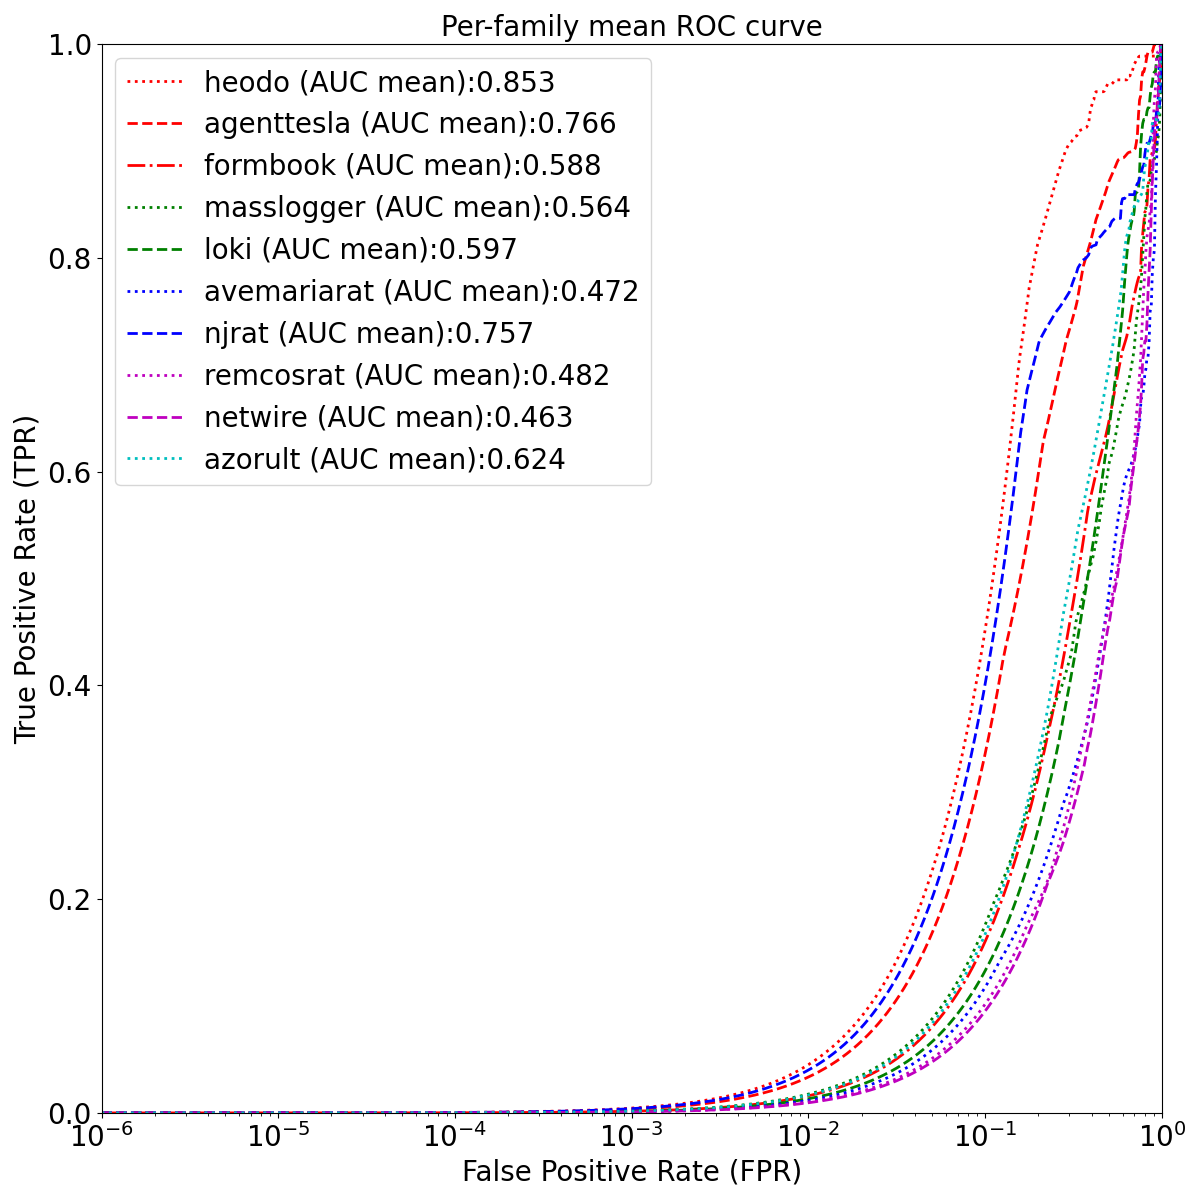
\includegraphics[width=0.6\textwidth]{./results/all_mean_fresh_roc_jointEmbedding.png}
        \vspace*{-0.2cm}
        \caption{Mean ROC curve and AUC statistics of \textBF{Joint Embedding} model for the prediction of all families on fresh dataset samples. The line represents the \textit{mean} TPR at a given FPR. Statistics were computed over \textBF{3} training runs, each with random parameter initialization.}
        \label{fig:allMeanFreshRocJointEmbedding}
    \end{figure}
}

\newcommand{\allMeanFreshRocProposedModel}{
    \begin{figure}[H]
        \vspace*{-0.5cm}
        \centering
        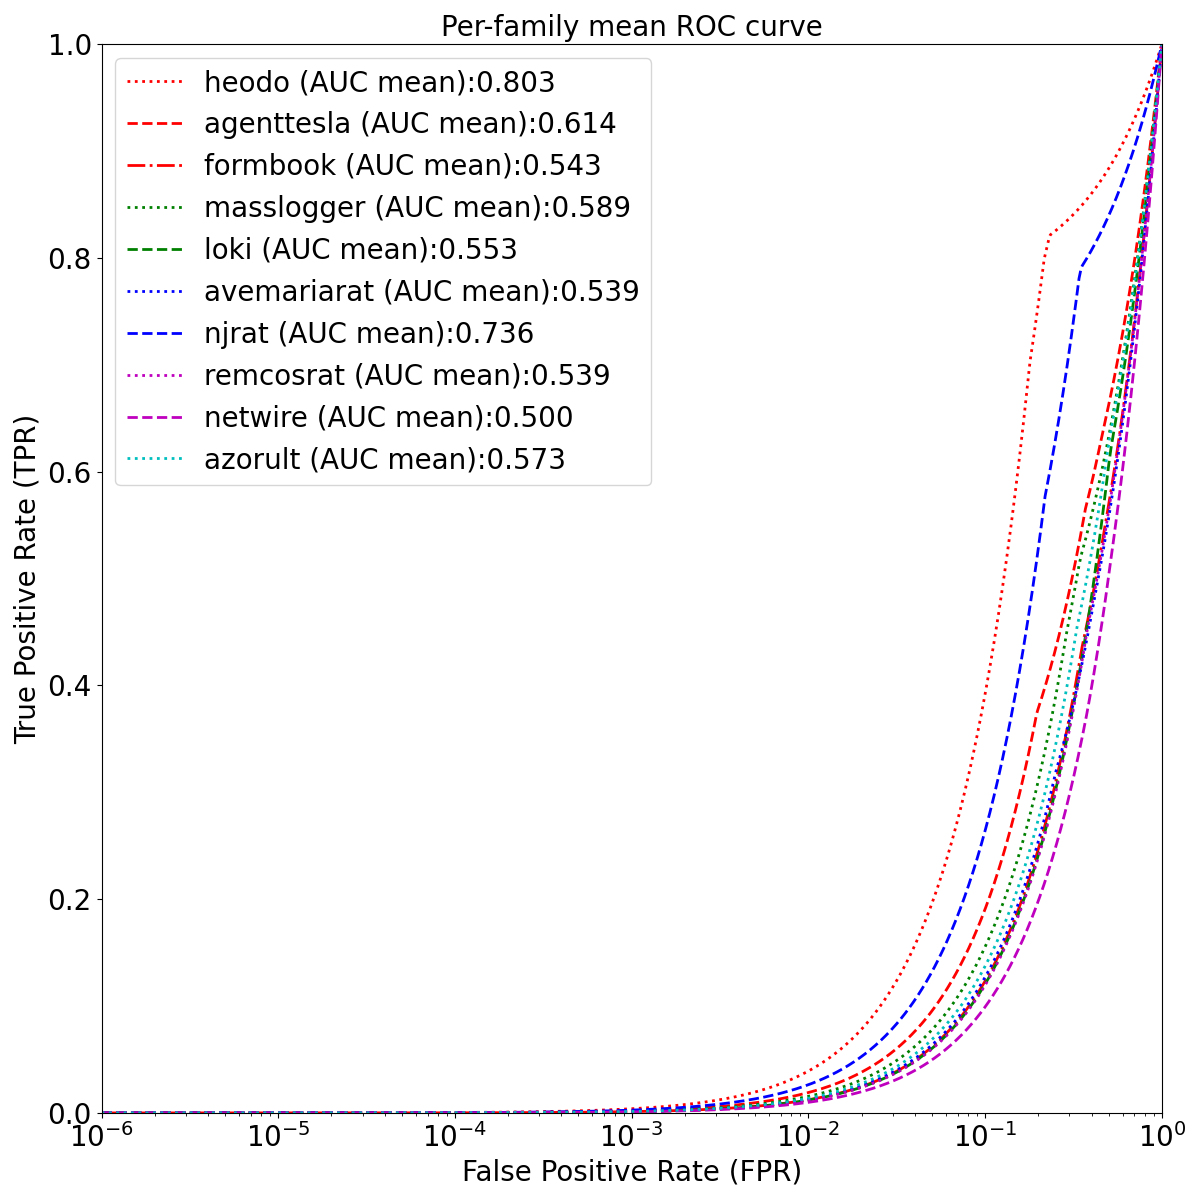
\includegraphics[width=0.6\textwidth]{./results/all_mean_fresh_roc_proposedModel.png}
        \vspace*{-0.2cm}
        \caption{Mean ROC curve and AUC statistics of \textBF{Proposed Model} for the prediction of all families on fresh dataset samples. The line represents the \textit{mean} TPR at a given FPR. Statistics were computed over \textBF{3} training runs, each with random parameter initialization.}
        \label{fig:allMeanFreshRocProposedModel}
    \end{figure}
}